\documentclass{article}
\usepackage{style-notes}

\newcounter{lecnum} 	% define counter for lecture number
\renewcommand{\thepage}{\thelecnum-\arabic{page}}	% define how page number is displayed (< lecture number > - < page number >)

% define lecture header and page numbers
% NOTE: to call use \lecture{< Lecture # >, < Lecture name >, < Chapter # >, < Chapter name >, < Section #s >}
\newcommand{\lecture}[5]{

    % define headers for first page
    \thispagestyle{empty} % removes page number from page where call is made

    \setcounter{lecnum}{#1}		% set lecture counter to argument specified

    % define header box
    \begin{center}
    \framebox{
      \vbox{\vspace{2mm}
    \hbox to 6.28in {\textbf{MATH 320: Probability} \hfill}
       \vspace{4mm}
       \hbox to 6.28in {{\hfill \Large{Lecture #1: #2} \hfill}}
       \vspace{2mm}
       \hbox to 6.28in {\hfill Chapters #3: #4 \small{(#5)}}
      \vspace{2mm}}
    }
    \end{center}
    \vspace{4mm}
    
    % define headers for subsequent pages
    \fancyhead[LE]{\textit{#2} \hfill \thepage} 		% set left header for even pages
    \fancyhead[RO]{\hfill \thepage}		% set right header for odd pages

}

% define macros (/shortcuts)
\newcommand{\bu}[1]{\textbf{\ul{#1}}}				% shortcut bold and underline text in one command
\newcommand{\blankul}[1]{\rule[-1.5mm]{#1}{0.15mm}}	% shortcut for blank underline, where the only option needed to specify is length (# and units (cm or mm, etc.)))
\newcommand{\vecinf}[1]{#1_1, #1_{2}, \ldots}		% define another vector of the form X_1, X_2, ....
\newcommand{\dx}[1]{\,\mathrm{d} #1}		% shortcut for dx after integral (variable x)
\newcommand{\integral}[4]{\displaystyle \int_{#1}^{#2} #3 \,\mathrm{d} #4}		% shortcut for large integral with limits and appending formatted dx (variable x)
\newcommand{\ddx}[1]{\frac{\mathrm{d}}{\mathrm{d} #1}\,}		% shortcut for derivative d/dx (variable x)

% NOTES on what didn't cover
% Theory lecture 5 end and start 6 -> valid cdf theorem and showing this via example, we only do valid pdfs and pmfs (probably because introduce pmf / pdf first, then cdf using those rather than vice versa like in theory)
% Theory lecture 6-2 -> identical random variables theorem and example where random variables are same but sample spaces are different (so still identical RVs cause they don't care about sample spaces)

\begin{document}

\lecture{8}{Distribution Functions}{2 and 3}{Distributions}{2.1 and 3.1}

\bu{Probability functions}\bigskip

Probabilities for discrete random variables\bigskip
\begin{itemize}
    \item Definition: The \textbf{probability mass function (pmf)} of a discrete random variable $X$ is given by
    \[f_X(x) = P(X = x), \quad \text{for all } x\]
    \item For a discrete random variable with a small number of outcomes, the pmf can be given in a table. When there is a very large or infinite number of possible outcomes, $f(x)$ can be given in a formula.
    \item Example: The number of injury claims per month is modeled by a random variable $N$ with
    \[P(N = n) = \frac{1}{(n + 1)(n + 2)},\quad\mbox{where $n \ge 0$.}\]\smallskip
    \begin{enumerate}[a)]
        \item Determine the probability of two claims.\vspace{80pt}
        \item Determine the probability of at most two claims.\vspace{80pt}
        \item Determine the probability of at least two claims.\vspace{80pt}
    \end{enumerate}
\end{itemize}\bigskip

Probabilities for continuous random variables\bigskip
\begin{itemize}
    \item For continuous random variables, does the pmf exist?
    \item[] These intervals are not countable, so we \blankul{1.5cm} use a pmf to assign probabilities.
    \item Instead, to find the general probability $P(a \le X \le b)$, we find the area bounded by $f(x)$ and the $x$-axis between $x = a$ and $x = b$ using integration.
    \item[] More specifically, we use a density function and find areas under the density function curve.
    \item Definition: A \textbf{probability density function (pdf)} is a continuous random variable $X$ is a real-valued function that can be used to find probabilities using
    \[P(a \le X \le b) = \integral{a}{b}{f(x)}{x}\]
    \item Notes:
    \begin{itemize}
        \item There is no probability associated with a single point:
        \item[] For $a \in {\cal X}, \hspace{10pt} P(X = a) = \integral{a}{a}{f(x)}{x} = 0$
        \item As a result: For any interval $(a, b)$, it doesn't matter if we include or exclude the endpoints in the continuous case (unlike with discrete).
        \item[] For $(a, b) \in {\cal X}, \hspace{10pt} P(a < X < b) =  P(a \le X \le b) =  \integral{a}{b}{f(x)}{x}$\vspace{30pt}
    \end{itemize}
    \item Example: Let $f(x) = \frac{1}{12}(x^2 + 1)$, \quad for $0 \le x \le 3$.
    \item[] Find: (a) $P(X \le 1)$ \hspace{50pt} (b) $P(X \ge 1)$ \hspace{50pt} (c) $P(0.5 \le X \le 1.5)$.\vspace{120pt}
\end{itemize}

Valid pmfs and pdfs\bigskip
\begin{itemize}
    \item There are rules that these new probability functions must follow, similar to the axioms our original probability assignments needed to satisfy.\bigskip
    \item Theorem: A function $f_X(x)$ is a pdf (or pmf) of a random variable $X$ if and only if
    \begin{enumerate}[(a)]
        \item  $f_X(x) \ge $ \hspace{10pt} for all $x$.
        \item $\displaystyle \sum_x f_X(x) = $ \hspace{10pt} (pmf) \hspace{20pt} or \hspace{20pt} $\integral{-\infty}{\infty} {f_X(x)}{x} = $ \hspace{10pt} (pdf). 
    \end{enumerate}
    \item Important note about $f(x)$ values.
    \begin{itemize}
        \item For the discrete case, $f(x)$ values were actually probabilities. \\ e.g. if $f(5) = 0.23$, there is a 23\% probability of $x = 5$.
        \item For the continuous case, the values of $f(x)$ are NOT probabilities themselves; they define areas which give probabilities.
        \item[] The values $f(x)$ must be positive, but they can be greater than 1.
        \item[] Example: Let $f(x) = 2, \quad 0 \le x \le 0.5$.
    \end{itemize}\bigskip
    \item Note these are why continuous variables use density functions and not mass functions. Cannot assign probability to every single point $\Longleftrightarrow$ Can't satisfy $\displaystyle \sum_{x \in {\cal X}} f(x) = 1$.\bigskip
    \item Examples:
    \begin{enumerate}
        \item Verify the pmf for $X$ is valid.\bigskip\\
        \begin{tabular}{| l | c | c | c | c |}
             \hline
             $x$ & 1 & 2 & 3 & 4\\
             \hline
             $f_X(x)$ & 0.43 & 0.12 & 0.3 & 0.15\\
             \hline
         \end{tabular}\vspace{40pt}
        \item Verify $f_X(x) = 2 x^{-3}, \quad 1 \le x < \infty$ is a valid pdf.\vspace{60pt}
        \item Let $X$ have the following pdf:
        \[
        f_X(x) =
            \left\{
            \begin{array}{ll}
                 cx^2 & 0 \le x \le 2\\
                 0 & \text{otherwise}
            \end{array}
            \right.
        \]
        \item[] Find the value of $c$ for which $f_X(x)$ is a valid pdf.\vspace{120pt}
    \end{enumerate}
\end{itemize}\bigskip

\bu{The cumulative distribution function}\bigskip

Concept of a cdf
\begin{itemize}
    \item Examples: Discrete case \hfill Continuous case\bigskip\\
    \begin{tabular}{| l | c | c | c | c |}
         \hline
         $x$ & 1 & 2 & 3 & 4\\
         \hline
         $f_X(x)$ & 0.43 & 0.12 & 0.3 & 0.15\\
         \hline
     \end{tabular}
     \hfill $f_X(x) = \frac{3}{8} x^2 \quad 0 \le x \le 2$\vspace{50pt}
     \item In these examples, probabilities were obtained by cumulatively adding successive probabilities in the table above or by accumulating more probability as we increased the upper bound.
    \item[] If we do this throughout the entire range of either case, we obtain the cumulative distribution function $F(x)$. Every random variable $X$ has an associated cumulative distribution function that can be defined as follows.
\end{itemize}\bigskip

Defining a cdf\bigskip
\begin{itemize}
    \item Definition: The \textbf{cumulative distribution function} or \textbf{cdf} of a random variable $X$, denoted $F_X(x)$, is defined by
    \[F_X(x) = P_X(X \le x),\quad\mbox{for all $x$.}\]
    \item Notes about $F(x)$: ALWAYS
    \begin{itemize}
        \item The cdf is defined for $-\infty < x < \infty$ always.
        \item The range of every cdf is $0 \le F(x) \le 1$ $\Longleftrightarrow$ Limits: 
        \item $F_X(x)$ is a non-decreasing function.
    \end{itemize}\bigskip
    \item DISCRETE case
    \item[] Example:
    \begin{enumerate}[(a)]
        \item Using the pmf table for $X$ below, find the cdf $F_X(x)$ as a table.\bigskip\\
        \begin{tabular}{| l | c | c | c | c |}
             \hline
             $x$ & 1 & 2 & 3 & 4\\
             \hline
             $f_X(x)$ & 0.43 & 0.12 & 0.3 & 0.15\\
             \hline
        \end{tabular}\vspace{30pt}
        \item Write $F_X(x)$ as a piecewise function:
        \item Plot the pmf and cdf.
        \begin{figure}[H]
            \center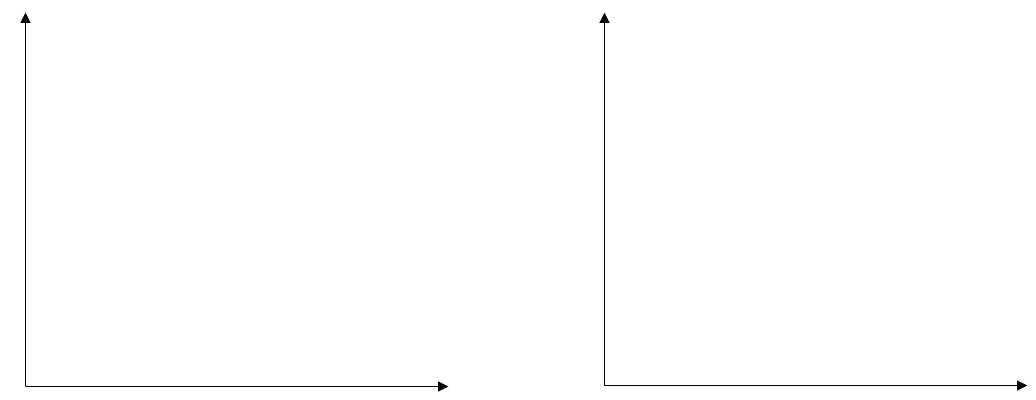
\includegraphics[scale=0.75]{test-2/two-plots}
        \end{figure}
    \end{enumerate}
    \begin{tabular}{l l l l}
        \ul{Observations of pmf} & & \ul{Properties of cdf} & \hspace{50pt}\\\\
        1) Sum of the heights = \blankul{1cm} & $\Longrightarrow$ & \hspace{50pt} \\\\\\
        2) Positive values (probabilities) only at \blankul{2cm} & $\Longrightarrow$ & \hspace{50pt}\\\\\\\\
        3) No probability \blankul{2cm} $x$ values &  $\Longrightarrow$ & \hspace{50pt}\\
     \end{tabular}\vspace{30pt}
    \item[] Properties
    \begin{itemize}
        \item The last entry in a table for $F(x)$ of a finite discrete random variable will always be 1.
        \item Even though $f(x)$ is only defined for certain values of $x$, we can define $F(x)$ for any real number.
        \item $F_X(x)$ is a right-continuous step-function.
    \end{itemize}\bigskip
    \item CONTINUOUS case
    \item[] Example: Let 
        \[
        f(x) =
            \left\{
            \begin{array}{ll}
                 \frac{3}{8} x^2 & 0 \le x \le 2\\
                 0 & \text{otherwise}
            \end{array}
            \right.
        \]
    \begin{enumerate}[(a)]
        \item Find the cdf $F(x)$.\vspace{150pt}
        \item Plot the pdf and cdf.\vspace{80pt}
    \end{enumerate}
    \begin{tabular}{l l l l}
        \ul{Observations of cdf} & & \ul{Properties of cdf} & \hspace{50pt}\\\\
        1) Plot starts at \blankul{1cm} and ends at \blankul{1cm} & $\Longrightarrow$ & \hspace{50pt} \\\\
        2) \blankul{3cm} at change points & $\Longrightarrow$ & \hspace{50pt}\\\\
     \end{tabular}
    \item[] Properties
    \begin{itemize}
        \item $F_X(\text{lower limit}) = 0$ and $F_X(\text{upper limit)} = 1$
        \item $F_X(x)$ is always a continuous function (even though the pdf $f_X(x)$ does not necessarily have to be continuous over $\mathbb{R}$).
    \end{itemize}\bigskip
    \item Types of random variables (another way to define).
    \begin{itemize}
        \item A random variable $X$ is \textbf{discrete} $\Longleftrightarrow$ $F_X(x)$ is a step function of $x$.
        \item A random variable $X$ is \textbf{continuous} $\Longleftrightarrow$ $F_X(x)$ is a continuous function of $x$.
    \end{itemize}
\end{itemize}\bigskip

Relationship between the cdf and pdf\bigskip
\begin{itemize}
    \item Since $F(x)$ is defined by integrating $f(x)$, it is clear that the derivative of $F(x)$ is $f(x)$. This simple relationship is very important when the derivative $F'(x)$ exists.
    \[F'(x) = f(x)\]
    \item Said another way: We can define the \textbf{pdf} of a continuous random variable $X$ as the function that satisfies
    \[F_X(x) = \integral{-\infty}{x}{f(t)}{t} \quad\quad \text{for all } x.\]
    \item[] Then using the Fundamental Theorem of Calculus, if $f_X(x)$ is continuous,
    \[\ddx{x} F_X(x) = f_X(x)\]
    \item This relationship means that the pdf (or pmf) contains the same information as the cdf. So knowing one of these about a random variable in very important and allows researchers to analyze it many, many ways.
    \item Example: Let $X$ have the following cdf:
    \[F(x) = P(X \le x) = 1 - \frac{1}{x^2}, \quad\quad 1 \le x < \infty\]
    \item[] Find the pdf $f(x)$.\vspace{100pt}
\end{itemize}\bigskip

Finding probabilities using the cdf\bigskip
\begin{itemize}
    \item ALWAYS
    \begin{itemize}
        \item Cdf gives a \blankul{2cm} probability.
       % \item Interval probabilities: $P(a \le X \le b) = F(b) - F(a)$
    \end{itemize}\bigskip
    \item DISCRETE case
    \begin{itemize}
        \item Cdf adds all probabilities of points less than or equal to $x$. Formula version of this for a particular value $x = a$:
        \[F(a) = P(X \le a) = \sum_{x \le a} f(x)\]
        \item The complement of this is:
        \[1 - F(x) = 1 - P(X \le x) = \hspace{50pt}\]
        \item[] which represents the probability $X$ is greater than $x$, \blankul{2cm}.\bigskip
        \item Interval probabilities: $P(a < X \le b) = P(X \le b) - P(X \le a) = F(b) - F(a)$\vspace{30pt}
    \end{itemize}\bigskip
    \item CONTINUOUS case
    \begin{itemize}
        \item Cdf accumulates all of the probability less than or equal to $x$, which means we are finding the probability up to $x$. So this $x$ the upper bound of the integral.
        \item[] To not confuse our letters, we change the letter of the variable  in the function being integrated (and in the differential $\text{d}t$).
        \[F_X(x) = \integral{-\infty}{x}{f(t)}{t}\]
        \item For a specific value of $x = a$, we find probability with
        \[F(a) = \integral{-\infty}{a}{f(x)}{x}\]
        \item The complement of this is:
        \[1 - F(a) = 1 - P(X \le a) = \hspace{50pt}\]
        \item Interval probabilities: $P(a \le X \le b) = P(X \le b) - P(X \le a) = F(b) - F(a)$
    \end{itemize}\vspace{20pt}
    \item Examples
    \begin{enumerate}
        \item Let $X$ have the cdf table below.\bigskip\\
        \begin{tabular}{| l | c | c | c | c | c |}
             \hline
             $x$ & 1 & 2 & 3 & 4 & 5\\
             \hline
             $F_X(x)$ & 0.16 & 0.63 & 0.67 & 0.78 & 1.00\\
             \hline
        \end{tabular}
        \item[] Find (a) $P(X \le 2)$ \hfill (b) $P(X > 3)$ \hfill (c) $P(X \ge 3)$ \hfill (d) $P(X < 4)$\vspace{70pt}
        \item[] (e) $P(2 \le X \le 4)$ \hspace{50pt} (f) $P(1 < X \le 5)$\vspace{70pt}
        \item Let $F_X(x) = \frac{x^3}{8}, \quad 0 \le x \le 2$.
        \item[] Find (a) $P(X \le 1)$ \hfill (b) $P(X < 1.5)$ \hfill (c) $P(X \ge1.25)$ \hfill (d) $P(X > 0.75)$\vspace{70pt}
        \item[] (e) $P(0.25 \le X \le 1)$ \hspace{50pt} (f) $P(1 < X \le 1.5)$\vspace{70pt}
    \end{enumerate}
\end{itemize}\bigskip

Examples\bigskip
\begin{itemize}
    \item Discrete
    \begin{enumerate}
        \item The cdf for the years until patients are asymptomatic for a certain disease is shown below:\smallskip
        \begin{center}
            \begin{tabular}{| l || c | c | c | c | c |}
            \hline
            Number of years $(x)$ & 1 & 2 & 3 & 4 & 5\\
            \hline
            $F(x)$ & 0.53 & 0.78 & 0.9 & 0.97 & 1.00\\
            \hline
            \end{tabular}
        \end{center}\bigskip
        \begin{enumerate}[a)]
            \item Find $P(X < 4)$ and $P(X = 3)$.\vspace{40pt}
            \item Write the piecewise functions of the pmf and cdf.\vspace{140pt}
            \item Plot a histogram of the pmf and a line graph of the cdf.\vspace{150pt}
        \end{enumerate}
    \end{enumerate}\newpage
    \item Continuous
    \item[] Straight-line densities
    \begin{enumerate}\setcounter{enumi}{1}
        \item Suppose we are offering a warranty insurance policy which pays for repairs on a new appliance. We know from experience that repair costs $X$ on a single policy will be on the interval $[0, 100]$, with probabilities highest for the lowest cost (\$0) and decreasing in a straight line fashion until $x$ reaches \$100.
        \begin{enumerate}
            \item Find an appropriate density function.\vspace{140pt}
            \item Calculate $P(X > 60)$.\vspace{130pt}
            \item Calculate $P(X \le 40)$.\vfill
        \end{enumerate}
        \begin{itemize}
            \item Conclusion: For straight-line densities, it is usually easier to find probabilities as areas of trapezoids or triangles.
        \end{itemize}
    \end{enumerate}\newpage
    \item[] Symmetric densities
    \begin{enumerate}\setcounter{enumi}{2}
        \item A risky investment has widely varying possible return percentages for next year. Best case: Return on investment (ROI) 100\% (doubles money by getting money invested back plus 100\% of the amount invested; Worst case: -100\% (loses all money invested).
        \item[] The percentage return is a random variable $X$ with that can be anywhere between the worst and best case, depending on the state of the economy. The pdf is:
        \[
        f(x) =
            \left\{
            \begin{array}{ll}
                 0.75(1 - x^2) & -1 \le x \le 1\\
                 0 & \text{otherwise}
            \end{array}
            \right.
        \]
        \begin{enumerate}
            \item Find the probability the investor has a ROI greater than 10\%.\vspace{100pt}
            \item Find the cdf $F(x)$; then find $P(X \ge 0.1)$.\vspace{130pt}
        \end{enumerate}
    \end{enumerate}
    \begin{itemize}
        \item This is actually a symmetric density, which means we have information about other probabilities as well just from finding the probability in part (b).
        \begin{align*}
            &P(X \ge 0.1) = \hspace{200pt} \\\\
            &P(0 < X < 0.1) = \\\\
            &P(-0.1< X <  0.1) = \\\\
            &P(\{X < -0.1\} \cup \{X > 0.1\}) = \\\\
        \end{align*}
    \end{itemize}\bigskip
    \item[] Piecewise densities
    \begin{enumerate}\setcounter{enumi}{3}
        \item The density function for a continuous random variable can be defined piecewise and fail to be continuous at some points. Let $X$ have the following pdf:
        \[
        f_X(x) =
            \left\{
            \begin{array}{ll}
                 0 & x < 0\\
                 560x & 0 \le x \le 0.05\\
                 -15x + 3.75 & 0.05 < x \le 0.25\\
                 0 & x > 0.25\\
            \end{array}
            \right.
        \]
        \begin{enumerate}
            \item Show that the total probability is 1.\vspace{220pt}
            \item Find $P(0.03 \le X \le 0.07)$.\vspace{220pt}\newpage
            \item Find the cdf $F_X(x)$.
            \item[] \textit{STRATEGY:} Find the cdf in cases.\bigskip\bigskip
            \item[] Case 1: $0 \le x \le 0.05 \hspace{20pt} \Longrightarrow \hspace{20pt} f(x) = 560x$\vspace{200pt}
            \item[] Case 2: $0.05 \le x \le 0.25 \hspace{20pt} \Longrightarrow \hspace{20pt} f(x) = -15x + 3.75$
        \end{enumerate}
    \end{enumerate}   
\end{itemize}


\end{document}